\chapter{Introduzione}

\subsubsection{What is an intelligent system (IS)}
\begin{center}
    \textit{a computer-based system that aims to replicate human cognitive abilities such as learning, perception, reasoning, and decision-making. }
\end{center}





\noindent By utilizing Machine Learning (ML), and other related technologies, these systems are capable of processing and analyzing data 
\hl{to perform tasks that typically require human intelligence}, make predictions, or provide insights.

\noindent Some examples of intelligent systems are:
\begin{itemize}
    \item virtual assistant like Siri and Alexa 
    \item autonomous vehicles 
    \item image recognition 
    \item fraud detection 
    \item \textit{and many others \dots}
\end{itemize}

\subsubsection{Diffusion and relevance}
In particular, ML allows us to \hl{process data at unprecedented scales}:
\begin{itemize}
    \item see patterns 
    \item detect problems earlier 
    \item allocate resources more effeciently
\end{itemize}

\newpage
\section{Major AI advancements \textcolor{blue}{[overview]}}

\subsubsection{Some recent improvements}
\begin{itemize}
    \item so-called \textbf{word embeddings} that are used as input to a Neural Network; it is 
    a set of techiniques in NLP where words are mapped to \textbf{vectors of real numbers}

    \begin{figure}[H]
        \centering
        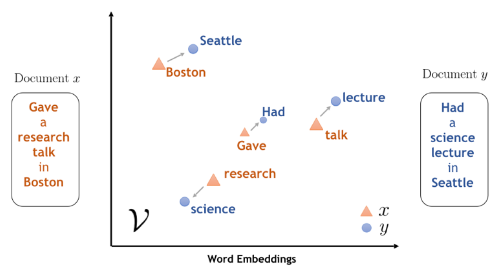
\includegraphics[width=0.6\linewidth]{01/images/word-embeddings.png}
    \end{figure}
    \item solving \textbf{analogy puzzles}
    
    \textit{Paris is to France as Tokyo is to \dots?}

    \texttt{Japan}
\end{itemize}

\subsection{Major AI advancements in the last 2 years}
AI has made significant progress across various domains, revolutionizing 
industries and starting to create profits\dots










